\clearpage
\section{典型例题与完整推导}
\label{sec:ch5-worked-examples}

\subsection{例题1：单臂与双臂应变桥的输出及灵敏度}
\keypoint{复习重点：微应变先换算；先求电阻变化，再分别代入精确桥路公式。}

\qs{从微应变到微伏、毫伏输出}{电阻应变片的初始阻值 $R=120\,\Omega$，灵敏系数 $S_g=2$；其余固定电阻初始也为 $120\,\Omega$，供桥电压 $U_0=3\,\mathrm V$，负载电阻视为无穷大。分别求 $\varepsilon=2\,\mu\varepsilon$、$2000\,\mu\varepsilon$ 时，单臂与相邻等量反向双臂电桥的输出，并比较灵敏度。}

\sol
采用本章桥臂编号，输出 $U_y=V_d-V_b$；单臂取 $R_1$ 增大，双臂取 $R_1$ 增大、$R_2$ 等量减小，因此对正应变均得到正输出。

\textbf{第一步：把应变换成电阻相对变化。}
\[
\delta=\frac{\Delta R}{R}=S_g\varepsilon.
\]
当 $\varepsilon=2\times10^{-6}$ 时，$\delta=4\times10^{-6}$、$\Delta R=0.00048\,\Omega$；当 $\varepsilon=2000\times10^{-6}=0.002$ 时，$\delta=0.004$、$\Delta R=0.48\,\Omega$。

\textbf{第二步：单臂采用精确分压式。}
\begin{align*}
U_{y,1}&=U_0\left(\frac{R+\Delta R}{2R+\Delta R}-\frac12\right)\\
&=\boxed{\frac{U_0\Delta R}{4R+2\Delta R}
=\frac{U_0\delta}{4+2\delta}}.
\end{align*}
代入两种应变：
\begin{align*}
U_{y,1}(2\,\mu\varepsilon)
&=\frac{3\times4\times10^{-6}}{4+8\times10^{-6}}\,\mathrm V
\approx\boxed{2.999994\,\mu\mathrm V},\\
U_{y,1}(2000\,\mu\varepsilon)
&=\frac{3\times0.004}{4+0.008}\,\mathrm V
\approx\boxed{2.994012\,\mathrm{mV}}.
\end{align*}
小信号近似 $U_{y,1}\approx U_0\delta/4$ 分别给出 $3\,\mu\mathrm V$ 与 $3\,\mathrm{mV}$。

\textbf{第三步：双臂让相邻电阻等量反向变化。}
\begin{align*}
U_{y,2}&=U_0\left(\frac{R+\Delta R}{(R+\Delta R)+(R-\Delta R)}-\frac12\right)\\
&=\boxed{\frac{U_0\Delta R}{2R}=\frac{U_0\delta}{2}}.
\end{align*}
分母精确保持 $2R$，所以无需舍去高阶项：
\[
\boxed{U_{y,2}(2\,\mu\varepsilon)=6\,\mu\mathrm V},\qquad
\boxed{U_{y,2}(2000\,\mu\varepsilon)=6\,\mathrm{mV}}.
\]

\begin{table}[H]
\centering\small
\begin{tabular}{@{}c c c c@{}}
\toprule
应变 & 单臂精确输出 & 单臂线性近似 & 双臂精确输出 \\
\midrule
$2\,\mu\varepsilon$ & $2.999994\,\mu\mathrm V$ & $3\,\mu\mathrm V$ & $6\,\mu\mathrm V$ \\
$2000\,\mu\varepsilon$ & $2.994012\,\mathrm{mV}$ & $3\,\mathrm{mV}$ & $6\,\mathrm{mV}$ \\
\bottomrule
\end{tabular}
\end{table}

\textbf{第四步：明确比较哪一种灵敏度。}零点小信号灵敏度为
\[
K_{\varepsilon,1}(0)=\frac{U_0S_g}{4}
=1.5\,\mathrm{\mu V}/\mu\varepsilon,
\qquad
K_{\varepsilon,2}=\frac{U_0S_g}{2}
=3\,\mathrm{\mu V}/\mu\varepsilon.
\]
双臂为单臂的2倍，并在理想等量反向条件下保持精确线性。若比较非零输入处的局部斜率，单臂应取导数：
\[
K_{\varepsilon,1}(\varepsilon)
=\frac{U_0S_g}{4(1+S_g\varepsilon/2)^2},\qquad
\frac{K_{\varepsilon,2}}{K_{\varepsilon,1}(\varepsilon)}
=2(1+S_g\varepsilon/2)^2.
\]
而 $U_y/\varepsilon$ 是从零点到测量点的\textbf{割线灵敏度}，对非线性单臂桥并不等于局部导数。直接比较两种输出的比值为 $U_{y,2}/U_{y,1}=2+\delta$，分别为 $2.000004$ 与 $2.004$；它与“零点灵敏度之比为2”并不矛盾。

\textbf{第五步：量化单臂桥路非线性。}以线性化输出为基准定义偏差
\[
e_{\mathrm{nl}}=\frac{U_{y,1}-U_{y,1}^{\mathrm{lin}}}{U_{y,1}^{\mathrm{lin}}}
=-\frac{\delta}{2+\delta}.
\]
两点分别约为 $-0.000200\%$ 与 $-0.199601\%$。若以精确输出为分母，线性近似的相对高估为 $\delta/2$，分别是 $0.000200\%$ 与 $0.200000\%$；误差分母不同，数值也略有不同。

\nt{此处双臂结果假定两片分别受等量拉、压应变。如果两片相邻且同向变化，理想输出会抵消。单臂桥输出的正负还取决于接线；换接输出端后，上述所有电压反号，灵敏度大小不变。}

\Needspace{8cm}
\subsection{例题2：全桥交流激励的输出与三组频谱}
\keypoint{复习重点：全桥的相邻臂必须等量反向；本题所有时间系数均为角频率。}

\qs{双频应变对正弦激励的调幅}{用四片电阻应变片组成全桥，测量
\[
\varepsilon(t)=A\cos10t+B\cos100t.
\]
激励电压为 $u_0(t)=E\sin10000t$，求电桥输出，并画出应变、激励与输出的频谱。各片灵敏系数相同，记为 $S_g$。}

\sol
\textbf{先说明全桥条件。}令 $\delta(t)=S_g\varepsilon(t)$，且
\[
R_1=R_3=R[1+\delta(t)],\qquad
R_2=R_4=R[1-\delta(t)].
\]
即一组对臂受拉、另一组对臂受等量压缩。代入桥路分压式：
\begin{align*}
u_y(t)&=u_0(t)\left[\frac{1+\delta(t)}2-\frac{1-\delta(t)}2\right]\\
&=\boxed{S_gE[A\cos10t+B\cos100t]\sin10000t}.
\end{align*}
该式在电阻--应变关系线性、四臂等量交替变化及高输入阻抗条件下为精确桥路结果。若四片同向等量变化，分压比均不变，不会得到此输出。

\textbf{展开乘积，直接读出四条正频率边带。}
\begin{align*}
u_y(t)=\frac{S_gEA}{2}\bigl[\sin10010t+\sin9990t\bigr]\\
\hspace{1.2cm}+\frac{S_gEB}{2}\bigl[\sin10100t+\sin9900t\bigr].
\end{align*}
注意这里用的是 $\sin\omega_ct\cos\Omega t$，且 $\omega_c>\Omega$，上下两边带均可写成正幅值正弦项。应变信号无直流分量，所以理想输出中\textbf{没有单独位于 $10000\,\mathrm{rad/s}$ 的载波线}。

\textbf{建立明确的双边谱线约定。}本题用复指数线谱
\[
v(t)=\sum_{\nu}C_{\nu}e^{\iu\nu t}
\]
表示周期信号，横轴为角频率 $\nu$。其中
\[
M\cos\nu t\ \longleftrightarrow\ C_{+\nu}=C_{-\nu}=\frac M2,
\]
\[
M\sin\nu t\ \longleftrightarrow\ C_{+\nu}=\frac{M}{2\iu}=-\iu\frac M2,
\quad C_{-\nu}=\iu\frac M2.
\]
若采用角频率傅里叶变换 $V_\omega(\omega)=\int v(t)e^{-\iu\omega t}\diff t$，则其冲激权重是 $2\pi C_\nu$，即
$V_\omega(\omega)=2\pi\sum_\nu C_\nu\delta(\omega-\nu)$。\textbf{谱线系数与傅里叶冲激权重不能混用。}

\begin{table}[H]
\centering\small
\begin{tabularx}{\linewidth}{@{}p{1.25cm} p{3.7cm} X@{}}
\toprule
信号 & 正角频率 $\nu$（$\mathrm{rad/s}$） & 对应的正频率复系数 $C_{+\nu}$ \\
\midrule
应变 & $10$；$100$ & $A/2$；$B/2$ \\
激励 & $10000$ & $-\iu E/2$ \\
输出 & $9990,\ 10010$ & 两条均为 $-\iu S_gEA/4$ \\
输出 & $9900,\ 10100$ & 两条均为 $-\iu S_gEB/4$ \\
\bottomrule
\end{tabularx}
\end{table}
所有信号为实信号，故负频率系数由 $C_{-\nu}=C_{+\nu}^{*}$ 给出。若 $A,B,E,S_g>0$，应变各线相位为零；激励及输出的正频率线相位均为 $-90^\circ$，负频率线为 $+90^\circ$。若 $A$ 或 $B$ 为负，相应谱线再反相 $180^\circ$。

\begin{center}
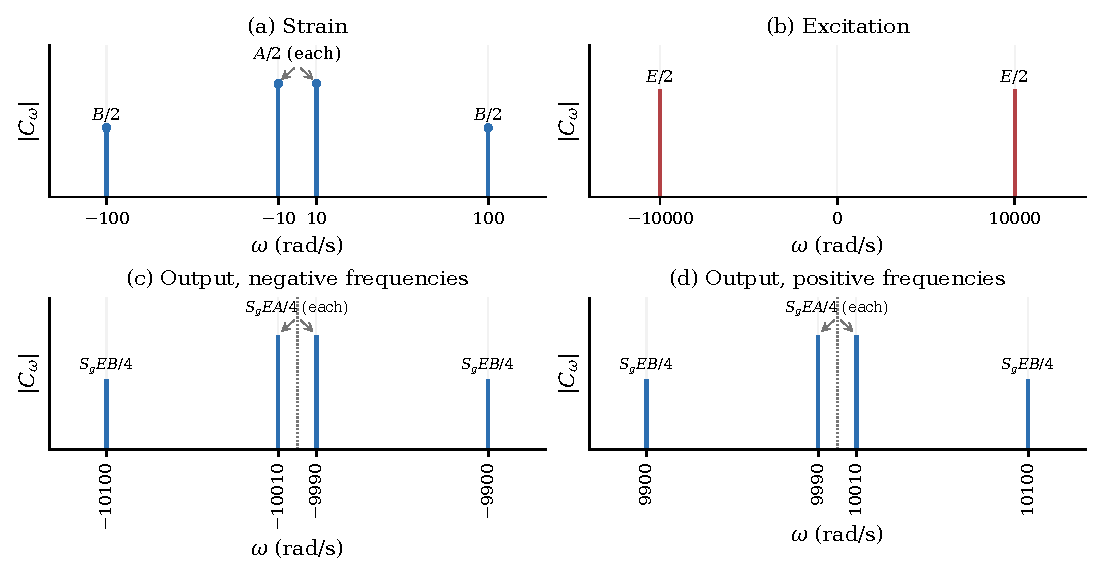
\includegraphics[width=.98\linewidth]{ch5-bridge-spectra.pdf}
\end{center}
图画的是双边复系数的模 $|C_\nu|$，纵向高度按符号示意，精确值见标注；输出正负频率簇分开展示，实际频率位置保持不变。虚线标出载频，虚线位置没有理想谱线。

\textbf{与Hz频谱的换算。}各频率都除以 $2\pi$。激励频率是
\[
f_c=\frac{10000}{2\pi}\approx1591.55\,\mathrm{Hz},
\]
并非 $10\,\mathrm{kHz}$。应变两频率约为 $1.592$、$15.915\,\mathrm{Hz}$，边带相对载频的偏移也分别是这两个数值。

\nt{只给单边峰值谱时，两组输出边带的高度分别为 $|S_gEA|/2$ 与 $|S_gEB|/2$。本题图采用双边复系数模，因此相应高度再减半。无论采用哪一种，都必须说明约定，并保留正弦激励所决定的相位信息。}

\clearpage
\subsection{例题3：带载波多频调幅的频率、幅值与频谱}
\keypoint{复习重点：括号中的直流产生载波，余弦分量各产生一对边带。}

\qs{从调幅表达式读取完整频谱}{已知
\[
x_a(t)=(100+30\cos\Omega t+20\cos3\Omega t)\cos\omega_ct,
\]
其中 $f_c=10\,\mathrm{kHz}$、$f_\Omega=500\,\mathrm{Hz}$。求各分量的频率与幅值，并画出调制信号与调幅波的频谱。}

\sol
把零均值的信息信号记为 $m(t)=30\cos\Omega t+20\cos3\Omega t$，把实际控制载波幅值的量记为 $q(t)=100+m(t)$。二者的区别只有 $q$ 含直流100；称“调制信号”时须明确指哪一个。

\textbf{第一步：展开为五个余弦。}
\begin{align*}
x_a(t)={}&100\cos\omega_ct\\
&+15\cos(\omega_c-\Omega)t+15\cos(\omega_c+\Omega)t\\
&+10\cos(\omega_c-3\Omega)t+10\cos(\omega_c+3\Omega)t.
\end{align*}
因此，$30$与$20$是信息信号的峰值，各自平均分到上下两个边带。

\begin{table}[H]
\centering
\begin{tabular}{@{}c c c@{}}
\toprule
分量 & 频率（$\mathrm{kHz}$） & 时域余弦峰值 \\
\midrule
三倍调制频率的下边带 & $10-1.5=8.5$ & $10$ \\
基频的下边带 & $10-0.5=9.5$ & $15$ \\
载波 & $10$ & $100$ \\
基频的上边带 & $10+0.5=10.5$ & $15$ \\
三倍调制频率的上边带 & $10+1.5=11.5$ & $10$ \\
\bottomrule
\end{tabular}
\end{table}

\textbf{第二步：给出带直流的调制量频谱。}沿用Hz傅里叶变换约定：
\[
Q(f)=100\delta(f)+15[\delta(f-500)+\delta(f+500)]
+10[\delta(f-1500)+\delta(f+1500)].
\]
若画的是 $m(t)$，删去 $100\delta(f)$，其余完全相同。调幅后
\begin{align*}
X_a(f)={}&50[\delta(f-10000)+\delta(f+10000)]\\
&+7.5\!\!\sum_{\nu\in\{9500,10500\}}[\delta(f-\nu)+\delta(f+\nu)]\\
&+5\!\!\sum_{\nu\in\{8500,11500\}}[\delta(f-\nu)+\delta(f+\nu)].
\end{align*}
每条正、负频率线的冲激权重是对应余弦峰值的一半；各系数为正，故相位均为零。

\begin{center}
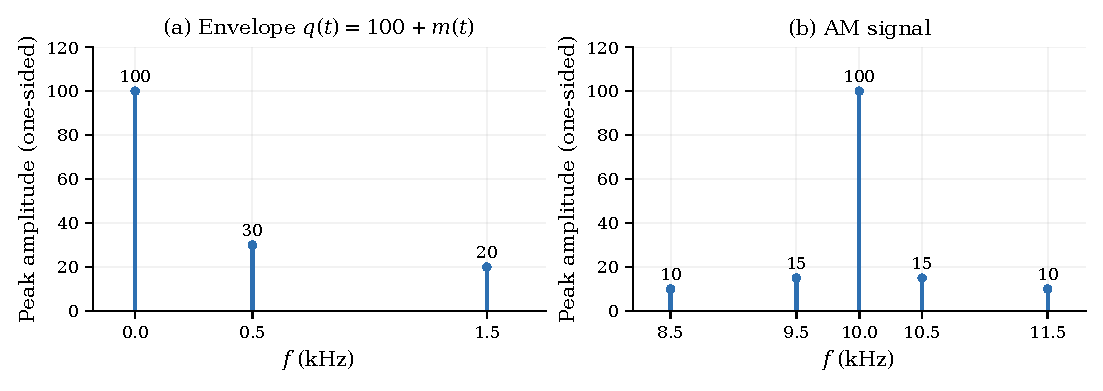
\includegraphics[width=.98\linewidth]{ch5-am-spectra.pdf}
\end{center}
为方便直接读取五个余弦的幅值，本图使用\textbf{单边峰值谱}：正频率余弦项画其峰值，直流画其常数值。若改画双边谱，在正负两侧各画一半峰值；直流仍为100，不做翻倍或减半。

\textbf{第三步：检验包络是否翻折。}由三角不等式，
\[
q(t)\geq100-30-20=50>0.
\]
因而该调幅波无包络翻折，可在适当时间常数与器件工作条件下采用包络检波，检出 $q(t)$ 后再去掉直流100。正频率占用范围为 $8.5\sim11.5\,\mathrm{kHz}$，带宽为 $3\,\mathrm{kHz}=2\times1500\,\mathrm{Hz}$。

\nt{直流100不产生“零频率的射频输出”，而是乘载波后形成 $10\,\mathrm{kHz}$ 谱线。$3\Omega$ 对应 $1500\,\mathrm{Hz}$，不能把它当作 $3\,\mathrm{Hz}$，也不能把两个边带幅值仍写成30、20。}

\subsection{例题4：10 kHz激励为何只测0--1500 Hz应变}
\keypoint{复习重点：载频是搬移位置，工作频率是可准确恢复的被测量频带。}

\qs{解释交流应变仪的频带标称}{某动态应变仪的电桥激励频率为 $10\,\mathrm{kHz}$，工作频率为 $0\sim1500\,\mathrm{Hz}$。用调幅与解调原理解释二者的关系。}

\sol
设应变频谱限于 $|f|\leq1500\,\mathrm{Hz}$，理想桥路输出 $u_y(t)=K\varepsilon(t)\cos(2\pi10000t)$，则
\[
U_y(f)=\frac K2[\mathcal E(f-10000)+\mathcal E(f+10000)].
\]
其中 $\mathcal E(f)$ 为应变频谱，$K$ 含桥路系数、片灵敏系数与激励幅值。因此输出在正载频附近占
\[
\boxed{10000-1500\leq f\leq10000+1500}
\quad\Longrightarrow\quad\boxed{8.5\sim11.5\,\mathrm{kHz}}.
\]
交流放大与带通环节应覆盖整段边带。同步乘以同相 $10\,\mathrm{kHz}$ 参考后，信号一部分回到 $0\sim1500\,\mathrm{Hz}$ 基带，另一部分移到 $20\,\mathrm{kHz}$ 附近。低通保留基带，再作比例标定，便得到应变输出。

所以\textbf{10 kHz是激励载频，1500 Hz是被测应变变化频率的上限}。工作频带受桥路、交流放大、解调和输出低通的整体幅相特性约束，并不是由激励频率直接等同得到。

\textbf{下限为何可为零？}恒定应变会改变载波幅值或相对相位，仍能由同步或相敏检波恢复为有正负的直流输出。只要测量链允许直流基带，就能测静态应变；信息不要求必须以低频电压直接通过全部交流放大级。

\textbf{带宽检查：}两边带共需3000 Hz带宽；输出低通还需在0--1500 Hz内满足精度，不能把1500 Hz直接当作无误差的 $-3\,\mathrm{dB}$ 截止点。

\clearpage
\subsection{例题5：截止频率、几何中心与倍频程判断}
\keypoint{复习重点：从 $f_{c2}/f_{c1}=2^n$ 推导，避免把三个不同的根号混淆。}

\qs{四个关于带通频带的命题}{设带通滤波器下、上截止频率为 $f_{c1},f_{c2}$，中心频率为 $f_0$。判断：
\begin{enumerate}
\item 一倍频程滤波器有 $f_{c2}=\sqrt2\,f_{c1}$。
\item $f_0=\sqrt{f_{c1}f_{c2}}$。
\item 截止频率位于幅值相对通带参考值下降约 $3\,\mathrm{dB}$ 的位置。
\item 下限频率相同时，一倍频程中心频率为 $1/3$ 倍频程中心频率的 $\sqrt[3]2$ 倍。
\end{enumerate}}

\sol
本题采用对数对称带通频带和常用半功率截止点约定。

\textbf{（1）错误。}一倍频程的定义是上下限频率之比为2：
\[
\boxed{f_{c2}=2f_{c1}},\qquad
f_0=\sqrt{f_{c1}\cdot2f_{c1}}=\sqrt2\,f_{c1}.
\]
命题把中心与下限之比，误写成上限与下限之比。若上、下限比为 $\sqrt2=2^{1/2}$，相应宽度只有半倍频程。

\textbf{（2）正确。}对数轴上的中点满足
\[
\log f_0=\frac{\log f_{c1}+\log f_{c2}}2,
\]
所以 $f_0=\sqrt{f_{c1}f_{c2}}$，不是算术平均 $(f_{c1}+f_{c2})/2$。该结论使用了本题的中心频率定义。

\textbf{（3）按本题常用约定正确。}半功率点的幅值比是 $1/\sqrt2$，
\[
20\log_{10}\frac{1}{\sqrt2}=-3.0103\,\mathrm{dB}\approx-3\,\mathrm{dB}.
\]
须相对于规定通带参考幅值；它不是绝对电压的分贝读数。采用其他截止指标的滤波器，需使用对应定义。

\textbf{（4）正确。}设共同下限为 $f_L$。一倍频程上限为 $2f_L$，中心为 $2^{1/2}f_L$；$1/3$ 倍频程上限为 $2^{1/3}f_L$，中心为 $2^{1/6}f_L$。故
\[
\boxed{\frac{f_{0,\,1\mathrm{oct}}}{f_{0,\,1/3\mathrm{oct}}}
=2^{1/2-1/6}=2^{1/3}=\sqrt[3]2}.
\]
例如共同下限100 Hz时，两中心频率分别为141.421 Hz和112.246 Hz，之比约1.25992。

\begin{focusbox}{三个根号各自表示什么}
一倍频程上、下限之比是 $2$；一倍频程中心与下限之比是 $\sqrt2$；相同下限的一倍频程中心与 $1/3$ 倍频程中心之比是 $\sqrt[3]2$。先写幂指数，再做相减，最不容易混淆。
\end{focusbox}

\clearpage
\subsection{\texorpdfstring{例题6：双频信号通过 $\tau=0.05$ s低通}{例题6：双频信号通过时间常数0.05 s的低通}}
\keypoint{复习重点：先计算两个 $\omega\tau$，系统相位差再加到原输入相位上。}

\qs{低通滤波前后幅值与相位的比较}{已知
\[
H(\iu\omega)=\frac1{1+\iu\omega\tau},\qquad\tau=0.05\,\mathrm s,
\]
输入 $x(t)=0.5\cos10t+0.2\cos(100t-45^\circ)$，求稳态输出，并比较输入、输出的幅相变化。}

\sol
系统静态增益为1，
\[
A(\omega)=\frac1{\sqrt{1+(0.05\omega)^2}},\qquad
\phi(\omega)=-\arctan(0.05\omega).
\]
对 $\omega_1=10\,\mathrm{rad/s}$，有 $\omega_1\tau=0.5$：
\[
A_1=\frac1{\sqrt{1.25}}=0.894427,
\quad\phi_1=-26.5651^\circ,
\]
\[
y_1(t)=0.5A_1\cos(10t+\phi_1)
=0.447214\cos(10t-26.5651^\circ).
\]
对 $\omega_2=100\,\mathrm{rad/s}$，有 $\omega_2\tau=5$：
\[
A_2=\frac1{\sqrt{26}}=0.196116,
\quad\phi_2=-78.6901^\circ.
\]
第二项原相位为 $-45^\circ$，因此输出总相位为 $-123.6901^\circ$：
\[
y_2(t)=0.2A_2\cos(100t-45^\circ+\phi_2)
=0.0392232\cos(100t-123.6901^\circ).
\]
叠加得到
\[
\boxed{\begin{aligned}
y_{\mathrm{ss}}(t)\approx{}&0.447214\cos(10t-26.5651^\circ)\\
&+0.0392232\cos(100t-123.6901^\circ).
\end{aligned}}
\]
常相位用角度标注，数值代入三角函数时应换成弧度。

\begin{table}[H]
\centering\small
\begin{tabular}{@{}c c c c c@{}}
\toprule
$\omega$（$\mathrm{rad/s}$） & 输入幅值 & 输出幅值 & 幅值衰减 & 系统新增相位差 \\
\midrule
$10$ & $0.5$ & $0.447214$ & $10.5573\%$ & $-26.5651^\circ$ \\
$100$ & $0.2$ & $0.0392232$ & $80.3884\%$ & $-78.6901^\circ$ \\
\bottomrule
\end{tabular}
\end{table}

\begin{center}
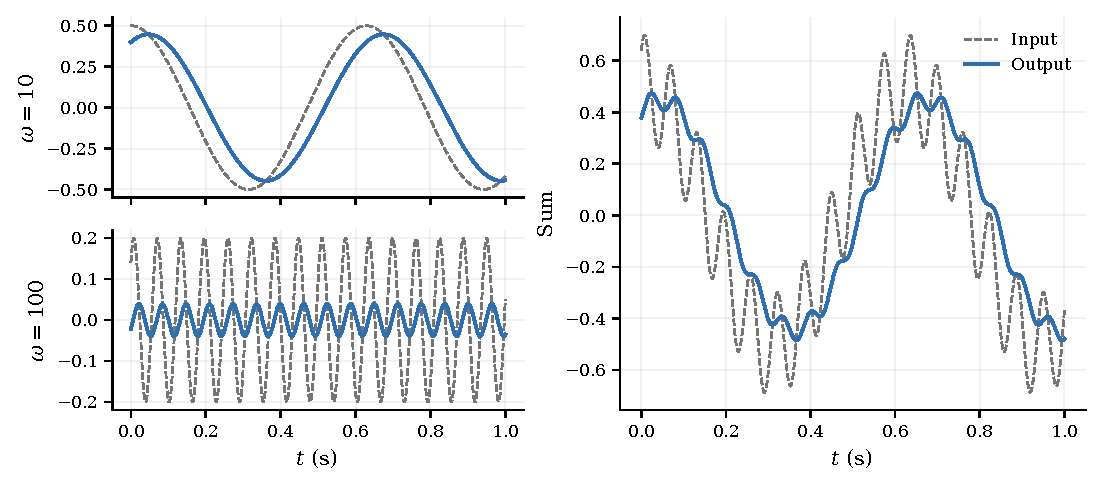
\includegraphics[width=.98\linewidth]{ch5-lowpass-example.pdf}
\end{center}
高频分量被明显抑制，输出主要由低频项决定。高、低频幅值比由 $0.2/0.5=0.4$ 变为约 $0.087706$；各分量相对强弱改变，叠加波形不能只用共同放大与延迟表示。

两分量的等效相位延迟也不同：
\[
t_1=\frac{\arctan0.5}{10}\approx0.046365\,\mathrm s,\qquad
t_2=\frac{\arctan5}{100}\approx0.013734\,\mathrm s.
\]
本滤波器截止角频率 $\omega_c=1/\tau=20\,\mathrm{rad/s}$，截止频率约 $3.1831\,\mathrm{Hz}$。输入高频项处于截止点之上，所以衰减显著。

\nt{这里 $\tau=0.05\,\mathrm s$，应直接代入本题参数。求的是稳定滤波后的稳态输出，不含启动暂态；若要求从零初始状态接入信号后的全过程，还应依据初始条件补上 $Ce^{-t/\tau}$。}
